
\section{Sequence Transformation}

\subsection{Abstraction and Reasoning Corpus: Additional Details and Examples}

In \cref{sec:sequence_transformation} of the main paper, we describe how ARC problems require reasoning about a range of different types of pattern operations---infilling, counting, translating and rotating shapes, and more. In \cref{fig:arc-successes}, we show sample problems among the 800 ARC problems for which text-davinci-003 correctly generalizes the pattern shown in a few train examples to a test example. In \cref{fig:arc-failures}, we show sample problems that are not correctly solved by text-davinci-003. In \cref{lst:arc-prompt}, we show an example context for an ARC problem encoded as integers.

\begin{figure}[h]
    \centering
    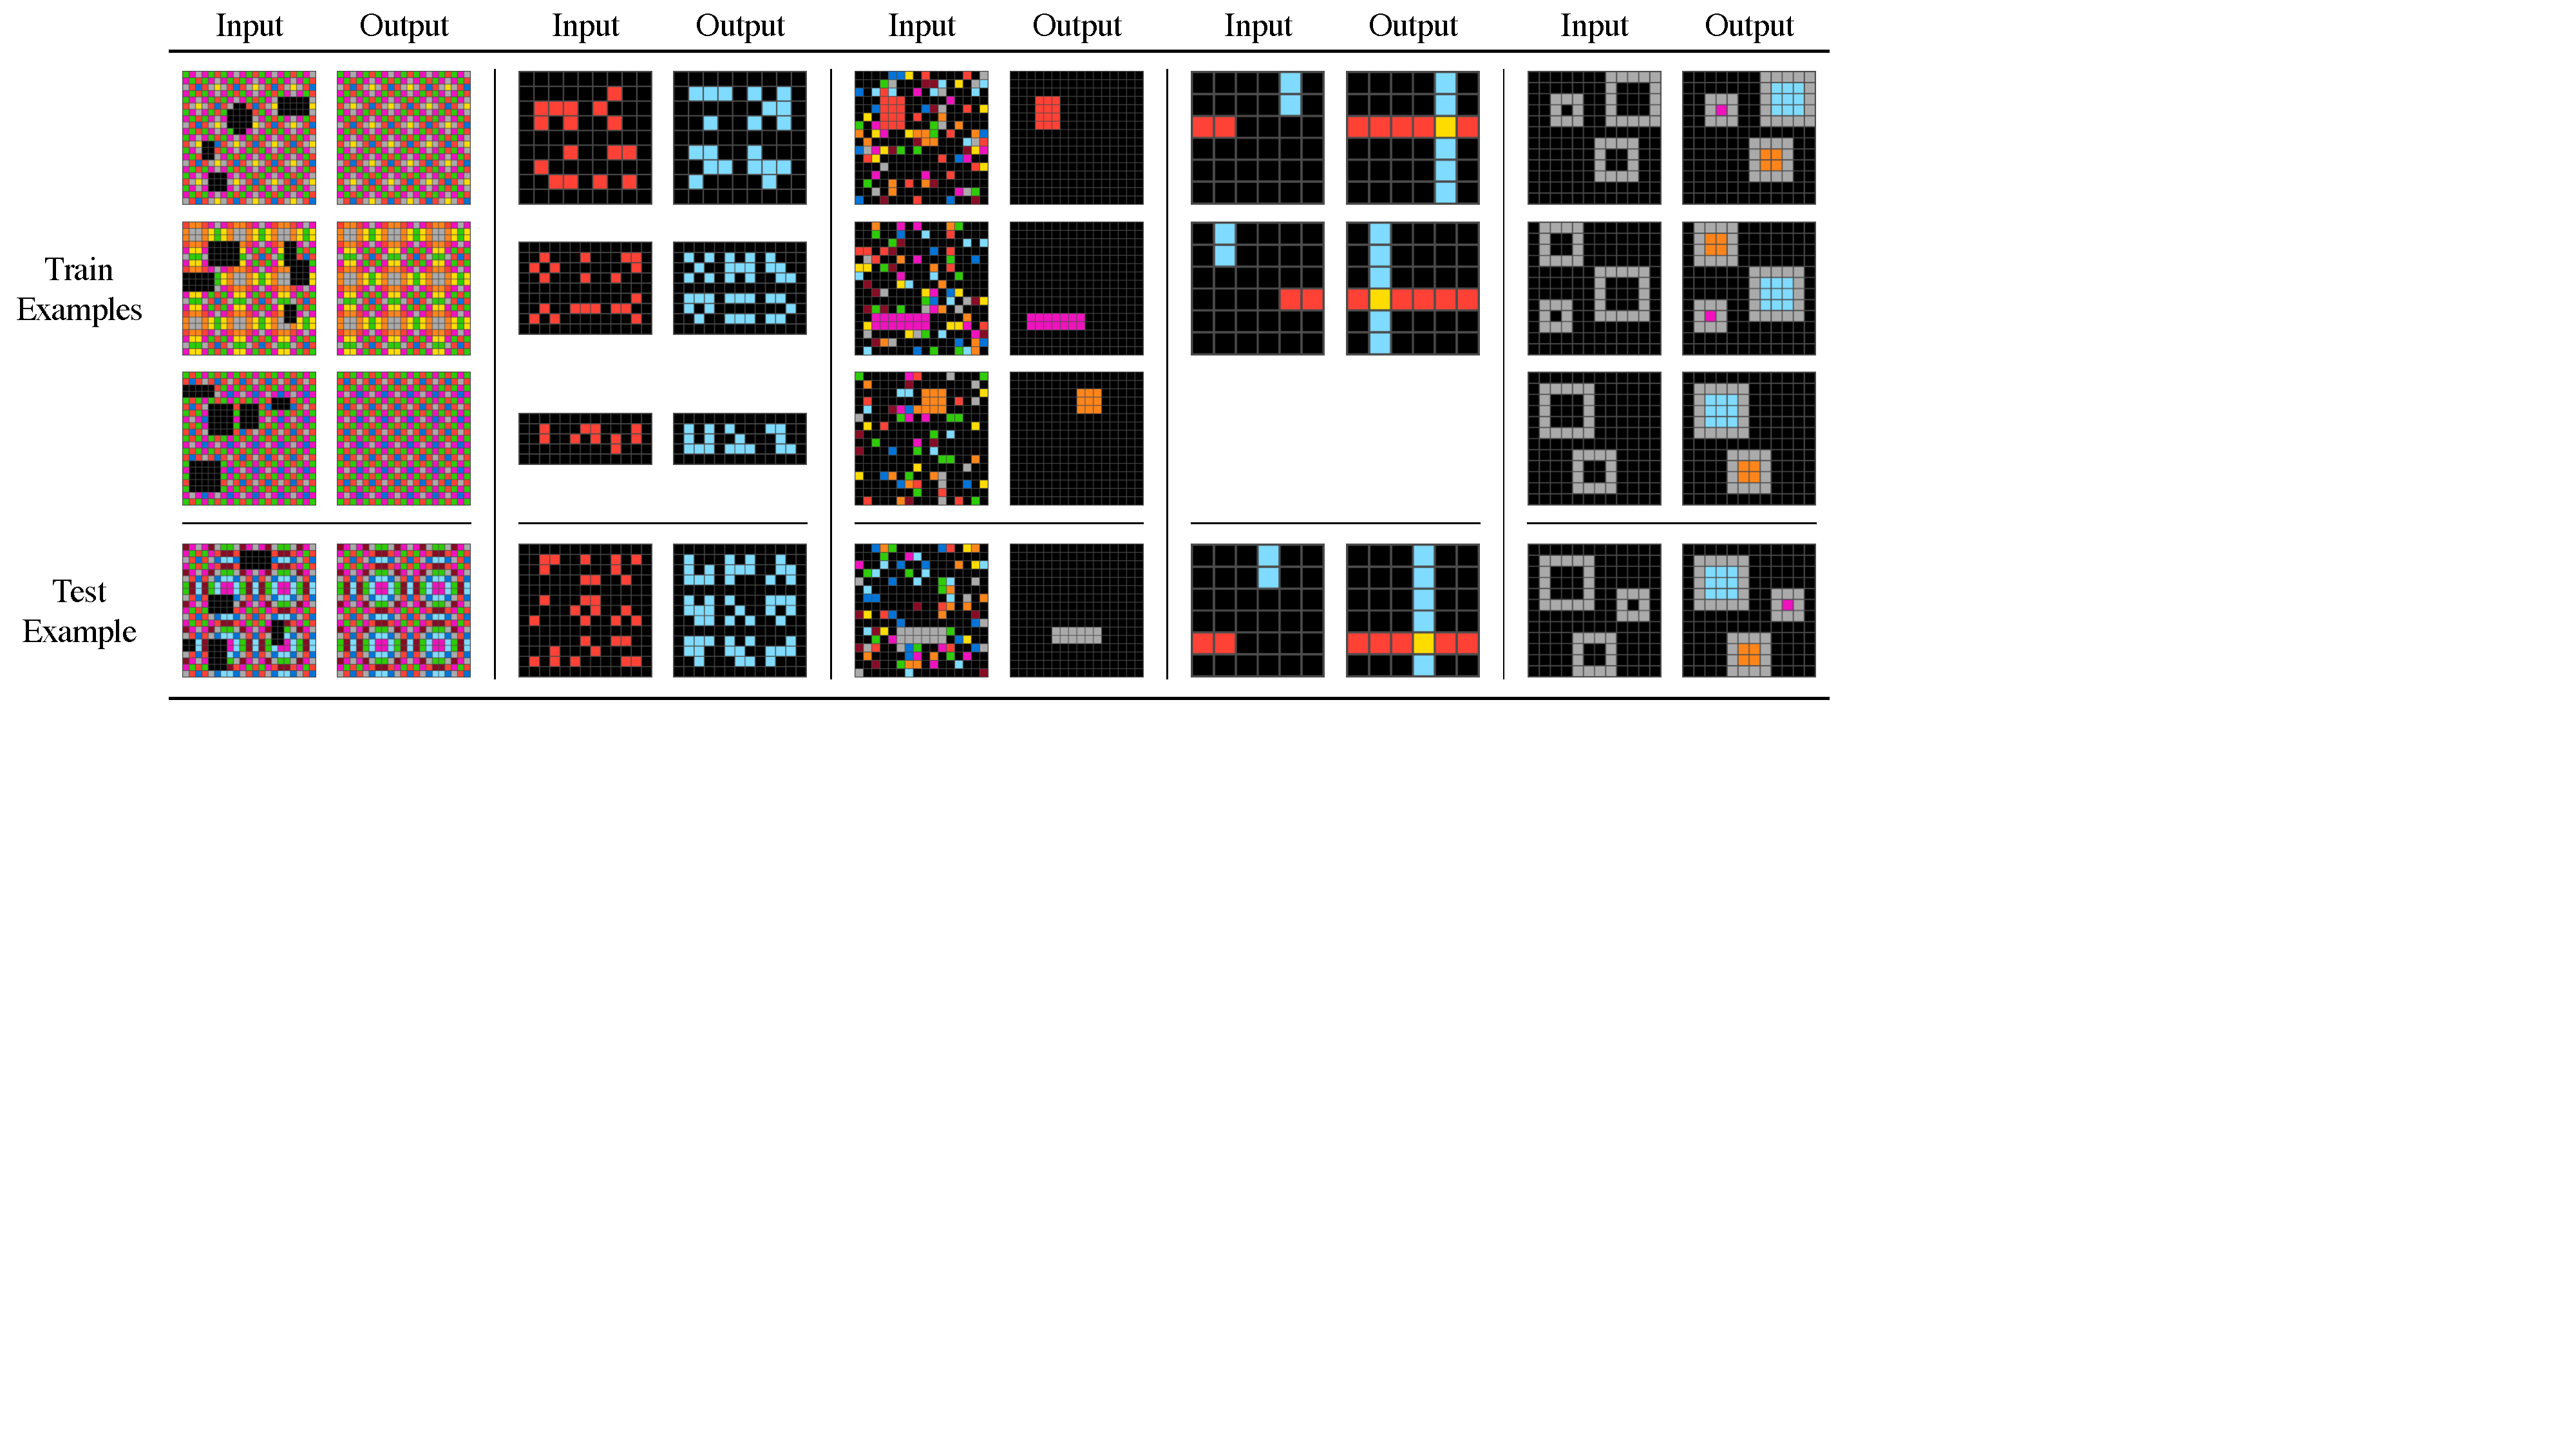
\includegraphics[width=\textwidth]{figures/arc-success-v1.pdf}
    \captionof{figure}{\small{Sample ARC problems that are correctly solved by text-davinci-003.}}
    \label{fig:arc-successes}
\end{figure}

\begin{figure}[h]
    \centering
    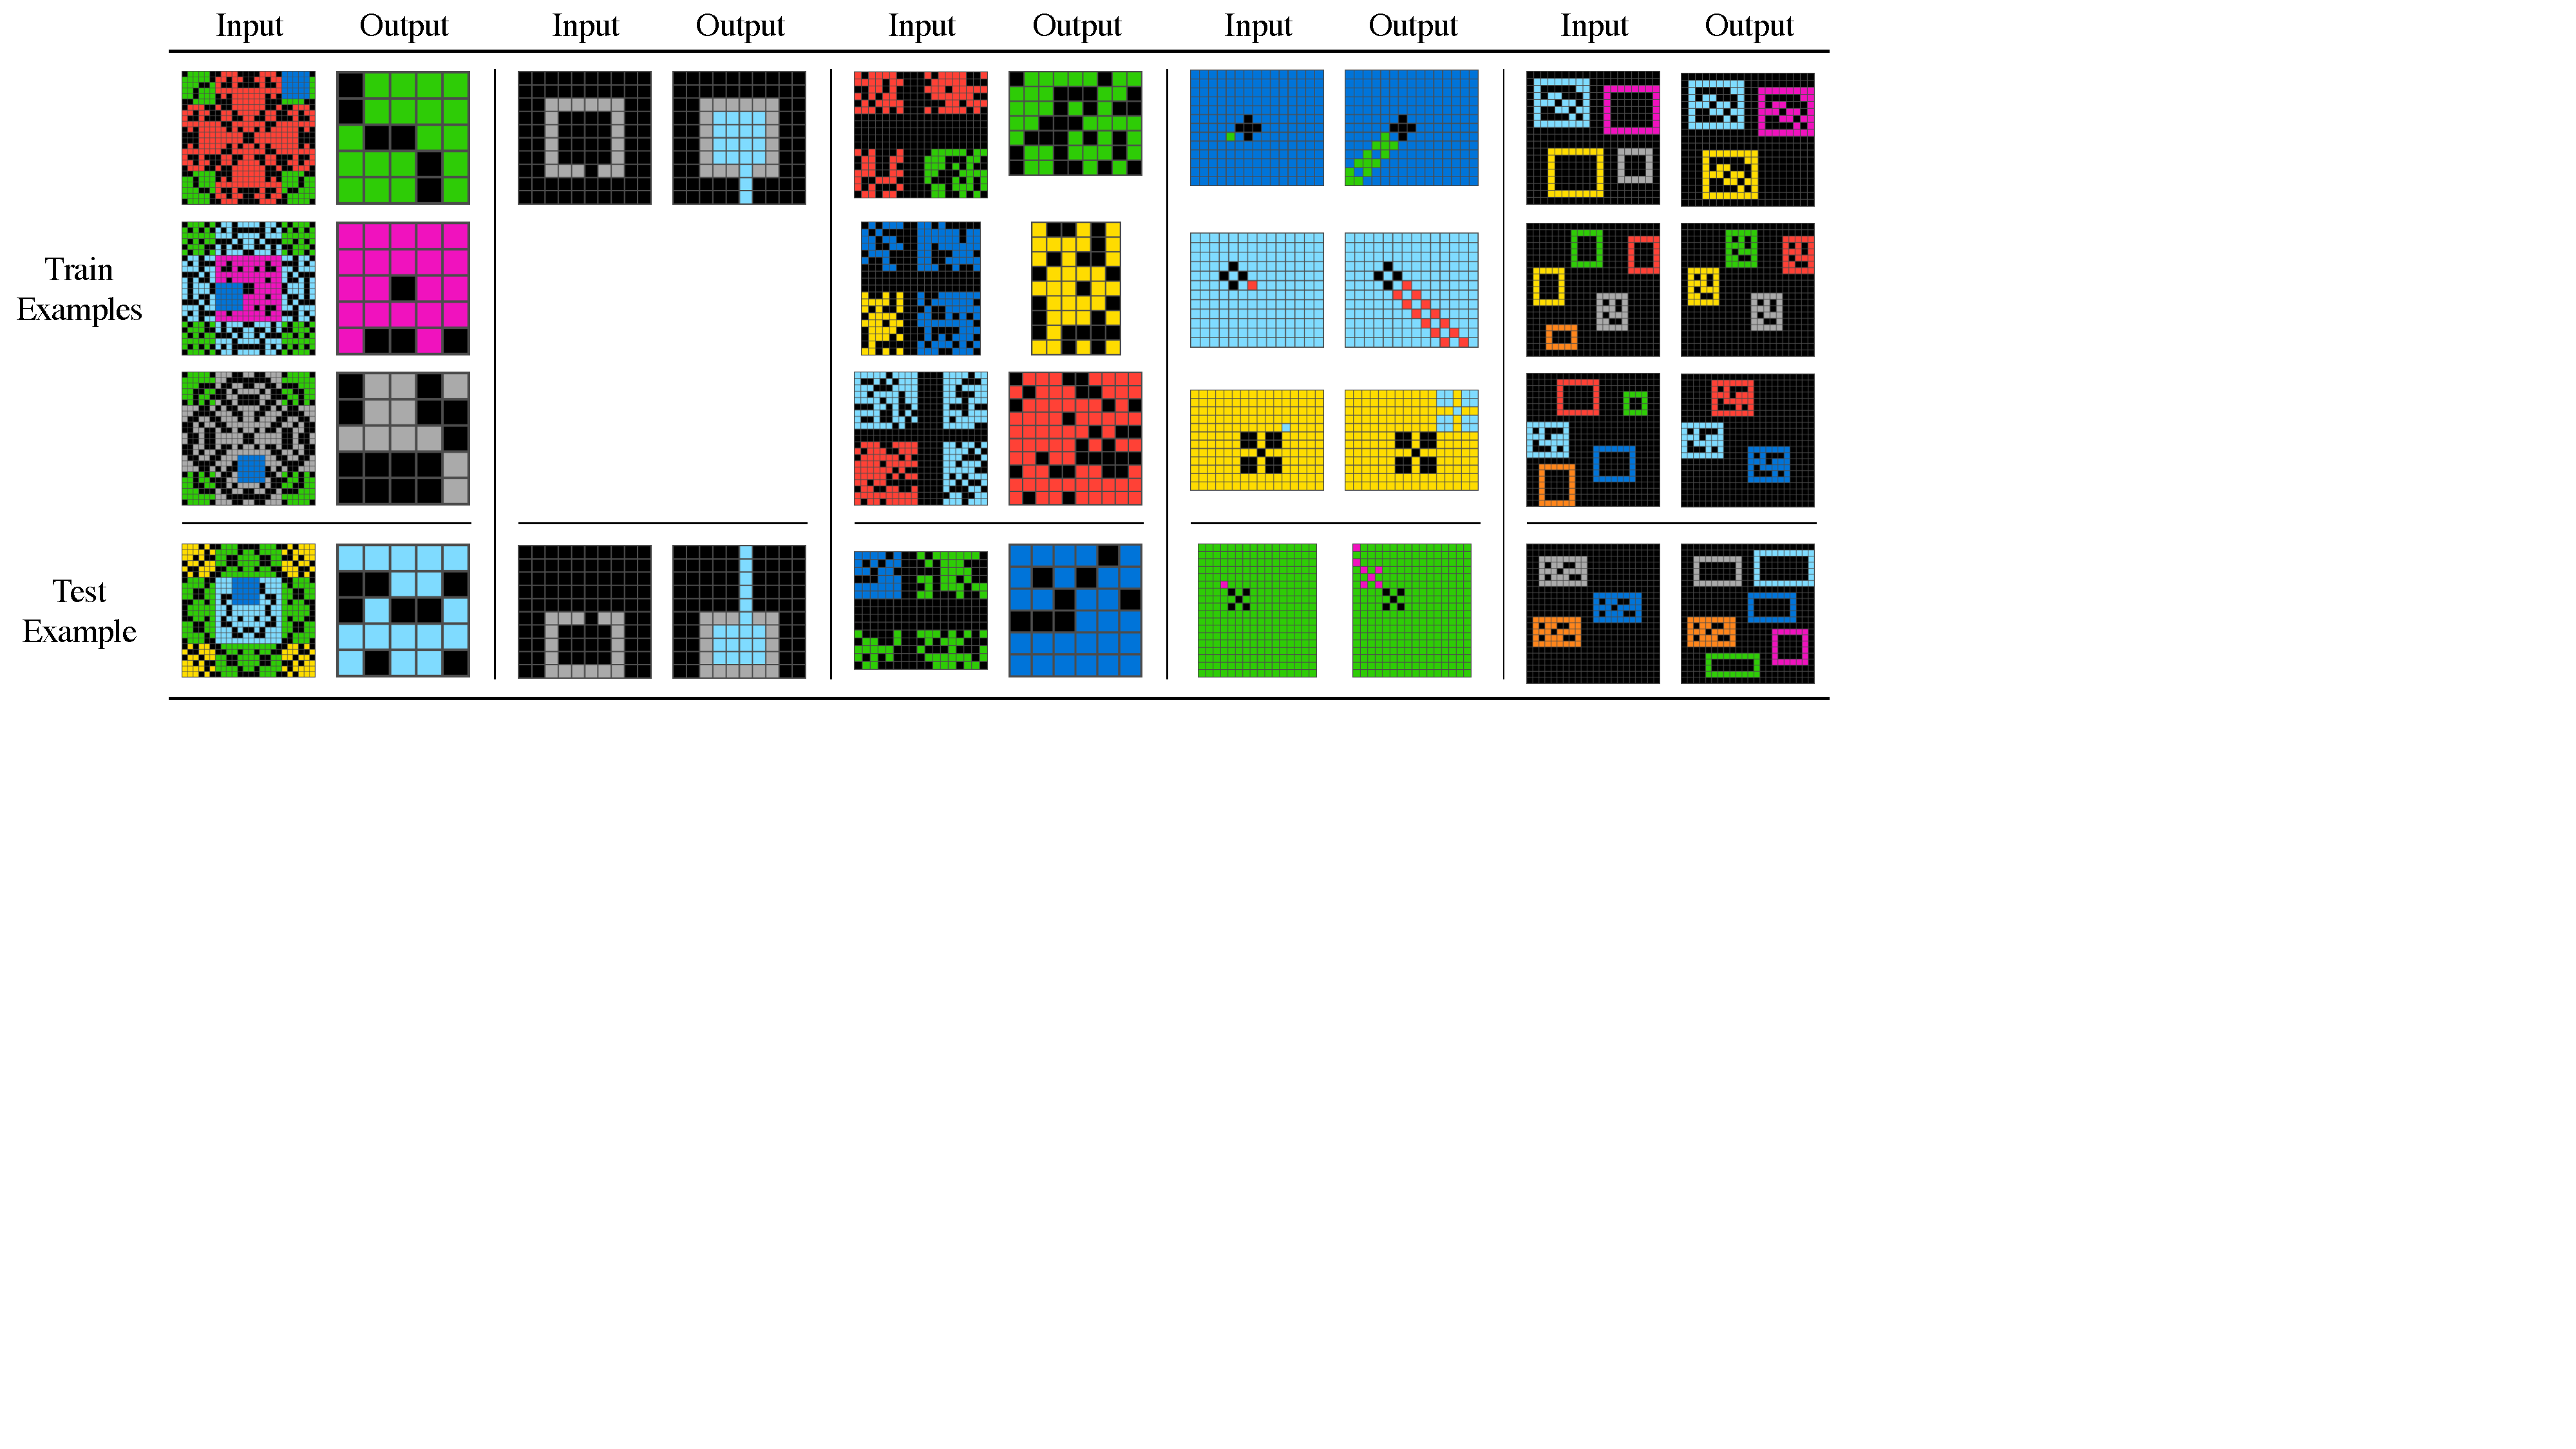
\includegraphics[width=\textwidth]{figures/arc-failure-v1.pdf}
    \captionof{figure}{\small{Sample ARC problems that are not correctly solved by text-davinci-003.}}
    \label{fig:arc-failures}
\end{figure}

\begin{lstlisting}[
    basicstyle=\ttfamily\footnotesize,
    backgroundcolor=\color{light},
    breaklines=true,
    caption={\small{Example context format for an ARC problem (only one input-output example is shown, along with a query input.}},
    captionpos=b,
    label={lst:arc-prompt}
    ]
input:
0, 0, 0, 0
0, 3, 4, 0
0, 7, 6, 0
0, 0, 0, 0
output:
3, 0, 0, 4
0, 0, 0, 4
0, 0, 0, 0
0, 0, 0, 0
7, 0, 0, 6
---
input:
0, 0, 0, 0
0, 5, 6, 0
0, 8, 3, 0
0, 0, 0, 0
output:
\end{lstlisting}

\subsection{Patterns over Low-Resolution Images}

In \cref{fig:picking}, we show an example in-context grasp detector which outputs target coordinates in a downsampled image, given 6 in-context examples, as well as an example of a simple forward dynamics model predicting spatial rearrangement of a red bowl into a green plate, given 9 in-context examples. As LLMs progress on the benchmarks discussed in Section \ref{sec:sequence_transformation}, they may become more robust and precise at performing such tasks.

\begin{figure}[h]

    \centering
    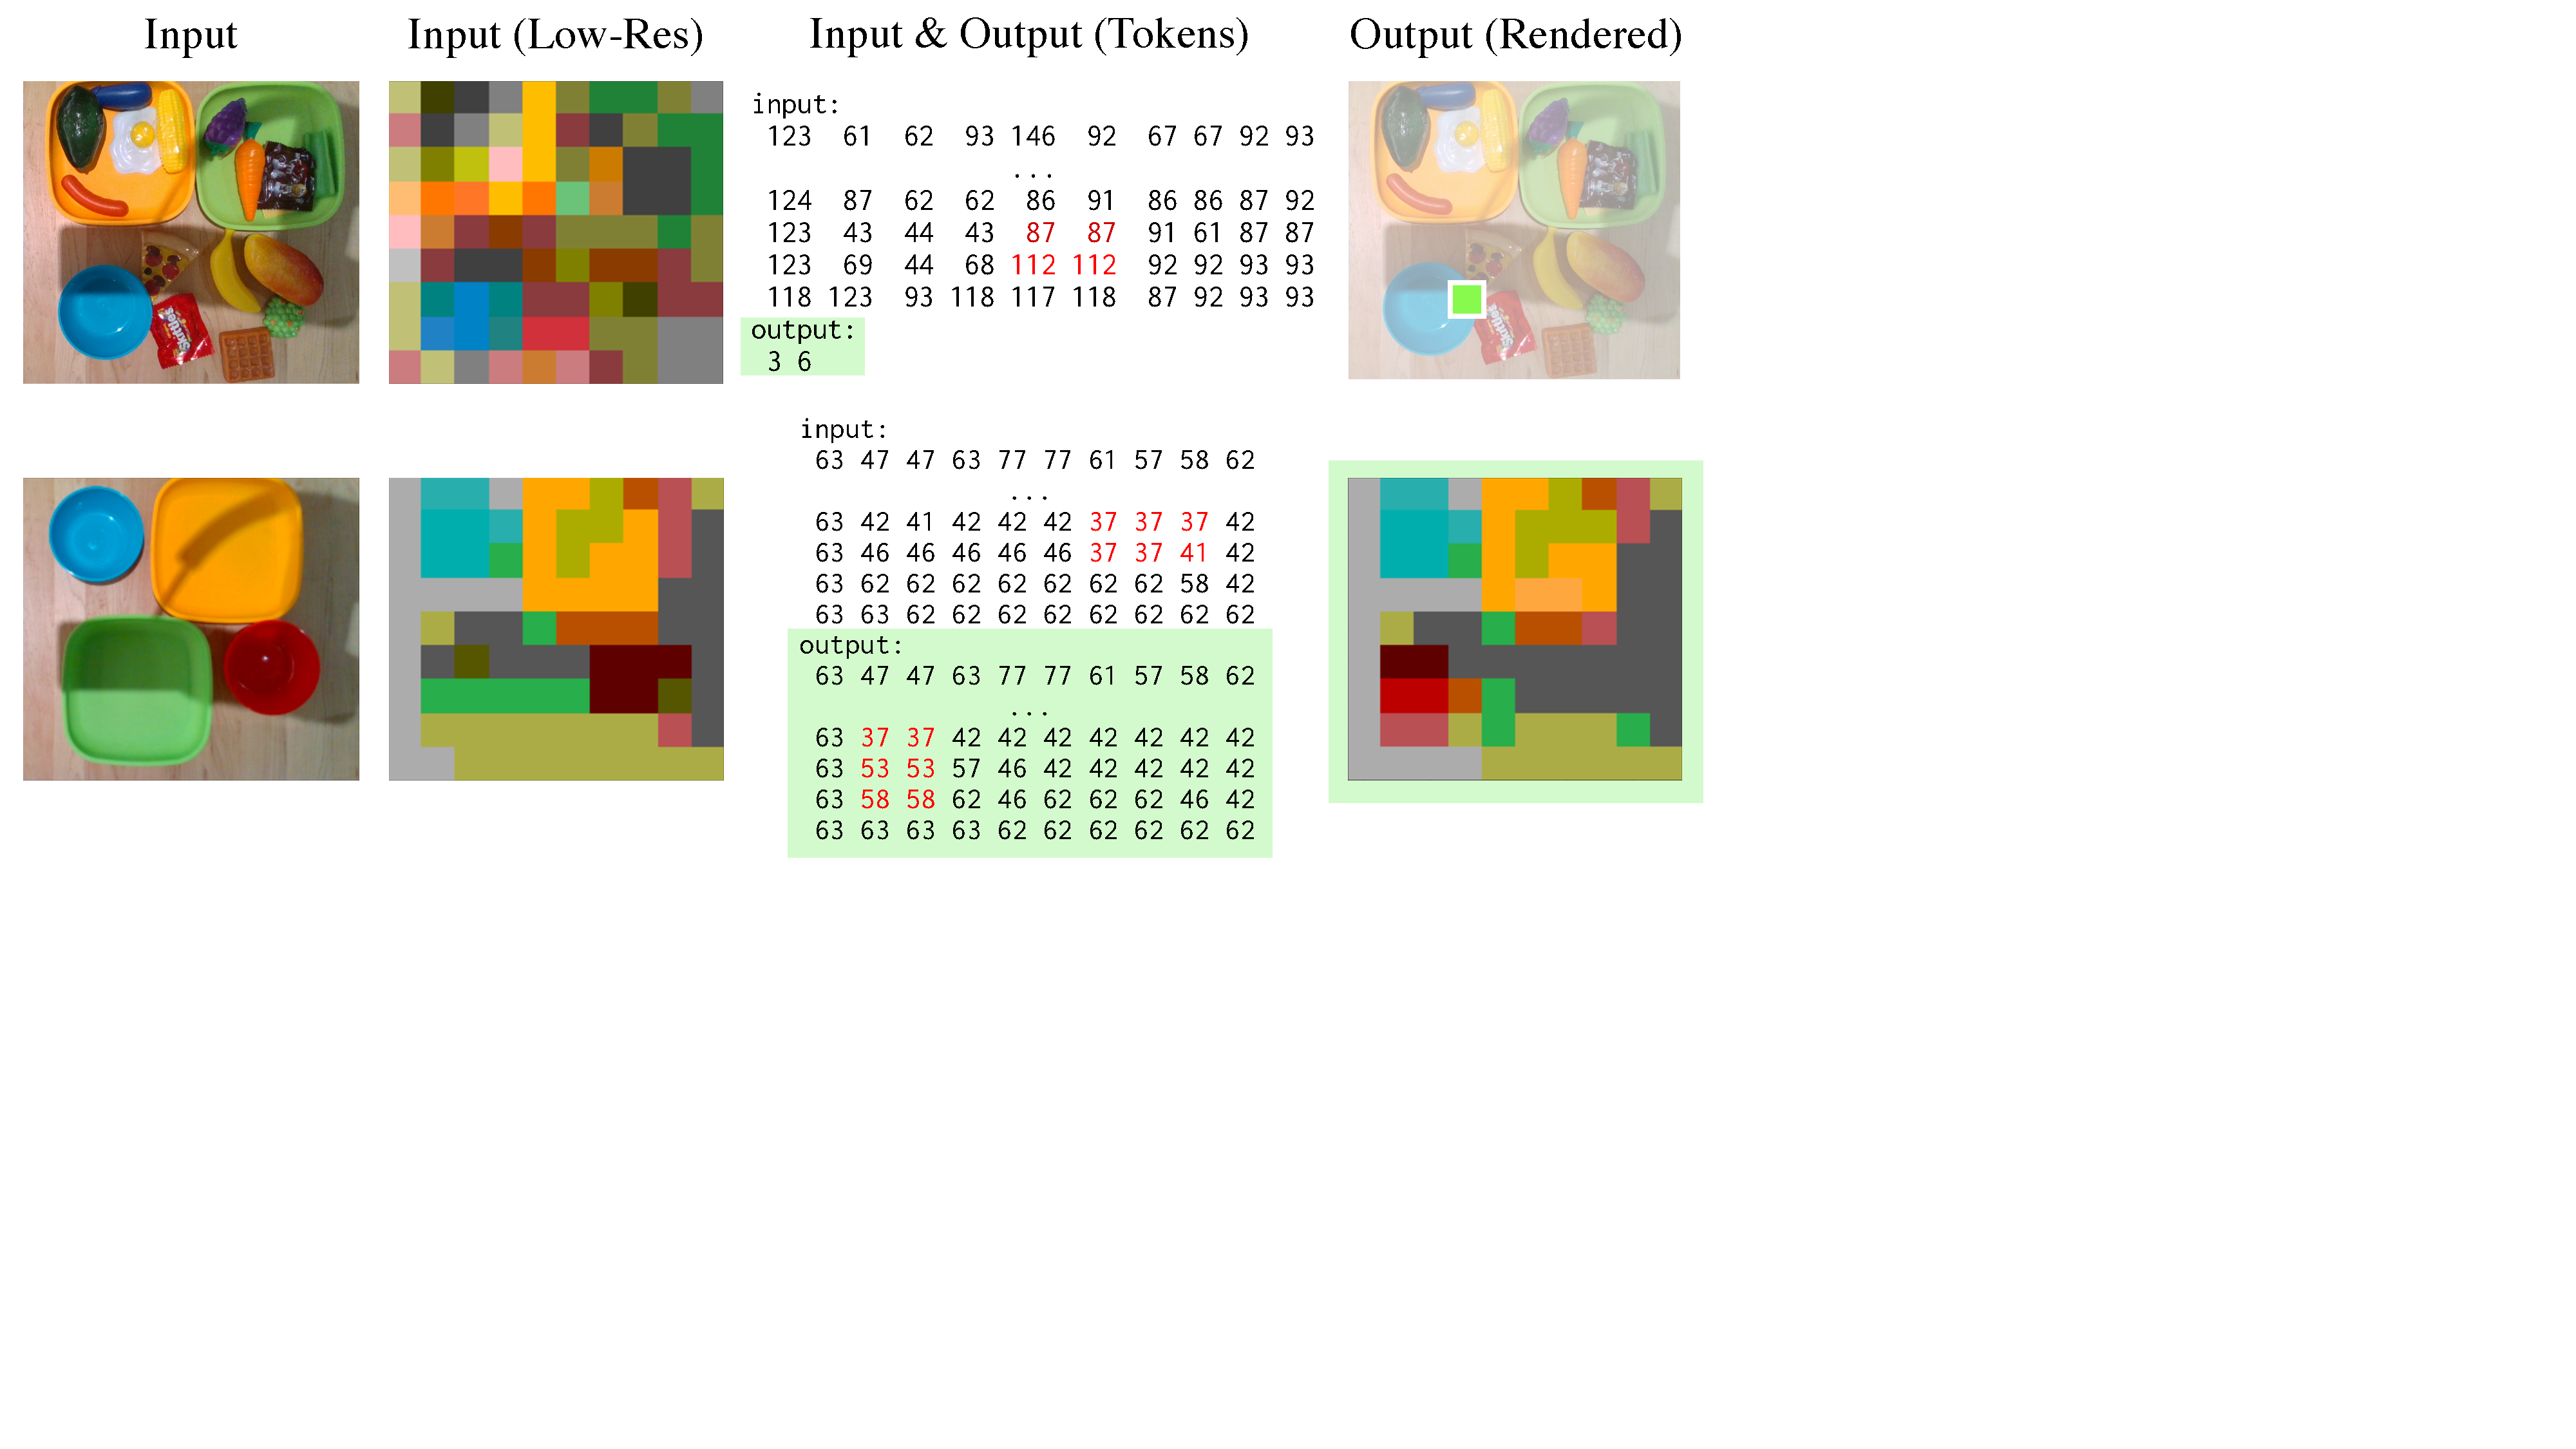
\includegraphics[width=0.7\textwidth]{figures/pick-rearrange.pdf}
    \caption{\small{Example LLM prediction as an in-context grasp detector (top) and a simple forward dynamics model (bottom).}
    }
    \label{fig:picking}
\end{figure}


\subsection{Token Invariance for New Token Embeddings}
\label{app:token-invariance-continuous}

In \cref{sec:sequence_transformation}, we have argued that LLMs are, to a certain extent, invariant to the choice of alphabet a pattern is encoded with, in line with prior work on mappings from semantically meaningful tokens to random tokens in a pre-trained language model \cite{min2022rethinking, pan2023context, paischer2022history}.
Here, we present an experiment that investigates token invariance even further by introducing new token embedding vectors the model has not seen during training.

We sample $K$ many new embedding vectors as Gaussian samples using the mean and 1 or 2 standard deviations of the original LLM embedding matrix statistics in each of embedding vector dimension.
This way, we create a new token embedding matrix, that mainly consists of the newly sampled token embeddings the model has not seen during training.
Additionally, we add embeddings from the original matrix that correspond to separating tokens (comma, period) to build the input prompts.
Although the model has never seen the new embedding vectors during training, we can feed them into the transformer as input and compute cosine similarities at the output analogously to how the original embedding matrix is treated.

\begin{figure}[h]
    \centering
    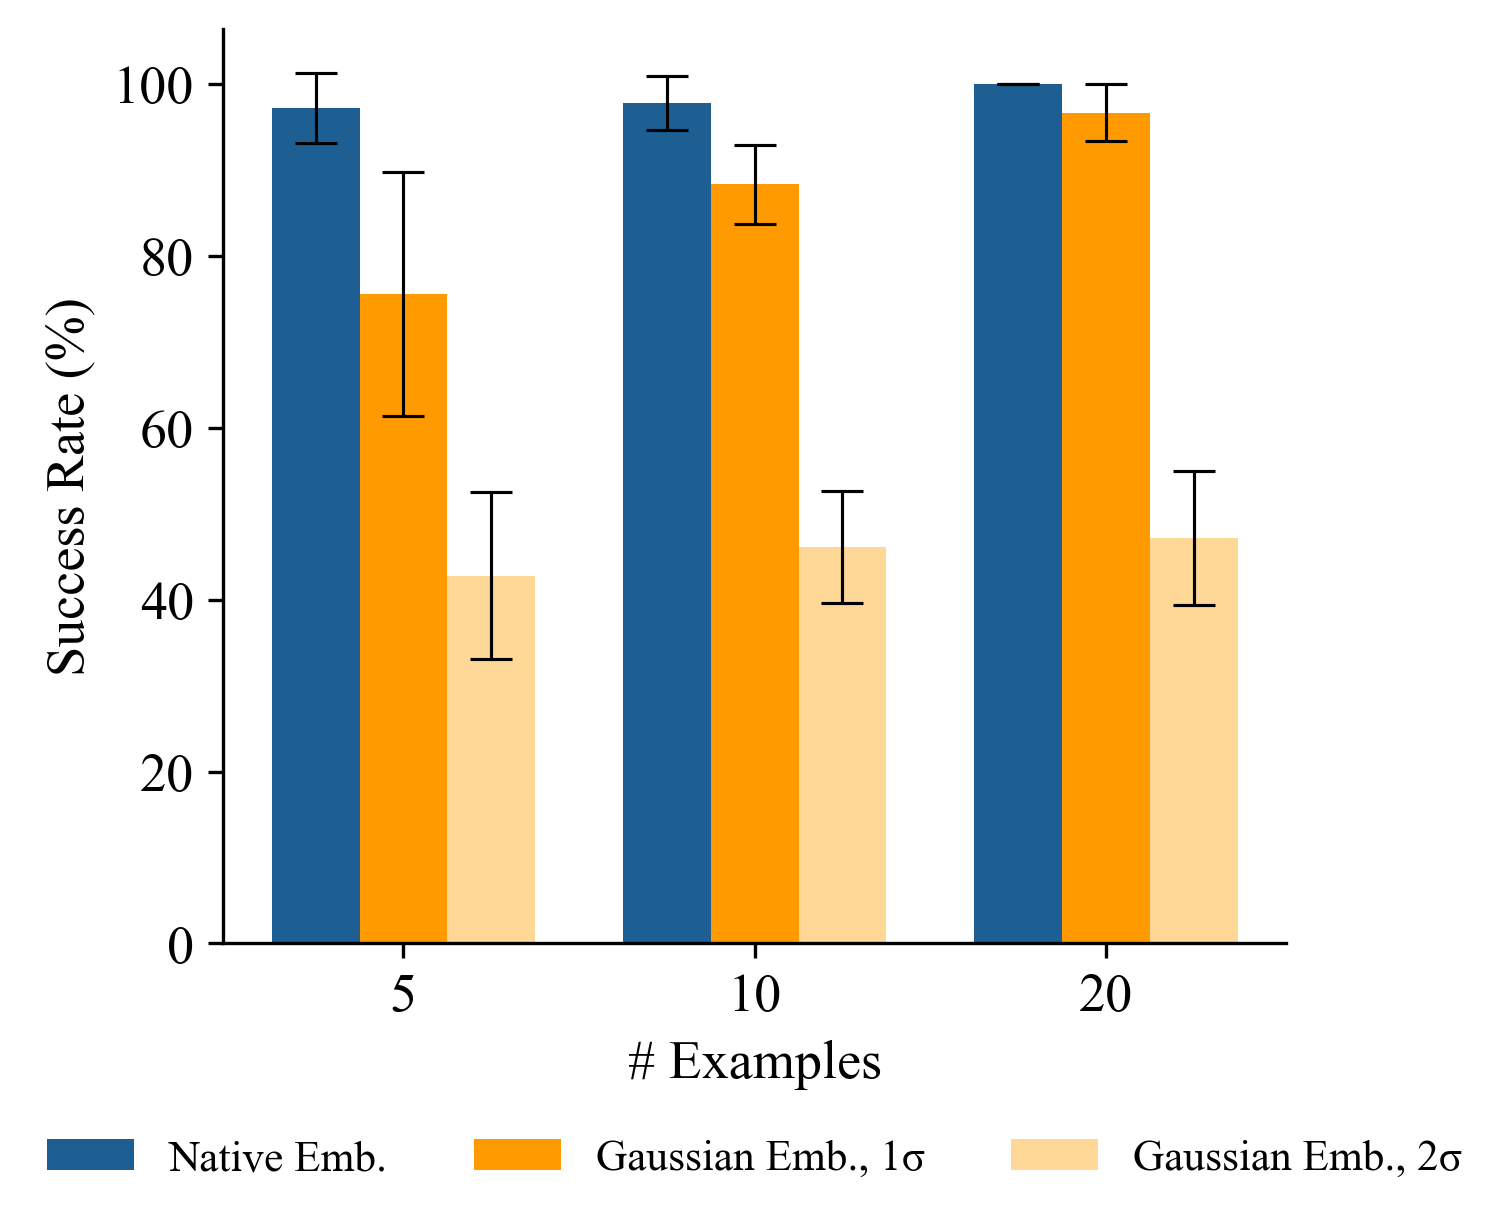
\includegraphics[width=8cm]{figures/continuous_tokens_v1.png}
    \caption{\small Token-invariance experiment with newly sampled token embeddings the model has not seen during training. Shown are success rates when using randomly sampled token embeddings from the native embedding matrix, or newly sampled embeddings. %
    }
    \label{fig:continuous_tokens}
\end{figure}

Fig.~\ref{fig:continuous_tokens} shows the success rate of correctly choosing the target token in a single-token prediction task when using the newly sampled embeddings in comparison with the native embedding matrix.
The tasks we are considering are of the form \tt{(1, 1, 2) $\mapsto$ 2} or \tt{(1, 2, 2) $\mapsto$ 1}.
We provide in-context examples to build a prompt of the form ``\tt{1, 2, 2, 1 ~\textbackslash n 3, 4, 4, 3 ~\textbackslash n 5, 6, 6, 5 ~\textbackslash n 7, 8, 8,}'' where the correct prediction should be ``\tt{7}'' in this example.
Note that the numbers ``\tt{1}'', ``\tt{2}'' etc. are randomly mapped to the newly sampled token embeddings for indexing purposes and in particular do not enter the LLM.
As one can see in Fig.~\ref{fig:continuous_tokens}, for $1\sigma$ noise sampling, the model is able to solve the task with the new embeddings with similar performance as with the native embeddings.
In case of $2\sigma$, the performance degrades.
Although these are relatively simple single-token prediction tasks, this experiment shows that LLMs show pattern recognition abilities even when prompted with out-of-distribution continuous input embeddings.
The results are obtained with $K=100$, averaged over 3 random seeds when sampling the token embeddings, 30 instances each, and a context length of 5, 10, or 20 examples. The LLM is the 8B parameter variant of \cite{chowdhery2022palm}.

\subsection{PCFG Benchmark: Additional Details and Ablations}
\label{app:pcfg-kw}

Our PCFG benchmark is a procedurally generated, adjustable-difficulty benchmark for measuring abstract sequence transformation capabilities in LLMs, based on the PCFG from \cite{hupkes2020compositionality}. In \cref{tab:pcfg-operators}, we show illustrations of the primitive operations in the PCFG that can be applied on one or two sequences of tokens. In \cref{tab:pcfg-examples}, we show examples of two transformations (of different complexities) from our benchmark, which are composed of the primitive operations.  In \cref{tab:pcfg-results-kw}, we show independent ablations of sequence length (number of tokens) $k$ and complexity (number of rules) $w$ in the sequence transformations, illustrating the way in which the solve rate decreases as either factor increases. In \cref{lst:pcfg-prompt}, we show an example context for a PCFG problem on integer sequences.

\begin{figure}[h]
    \centering
    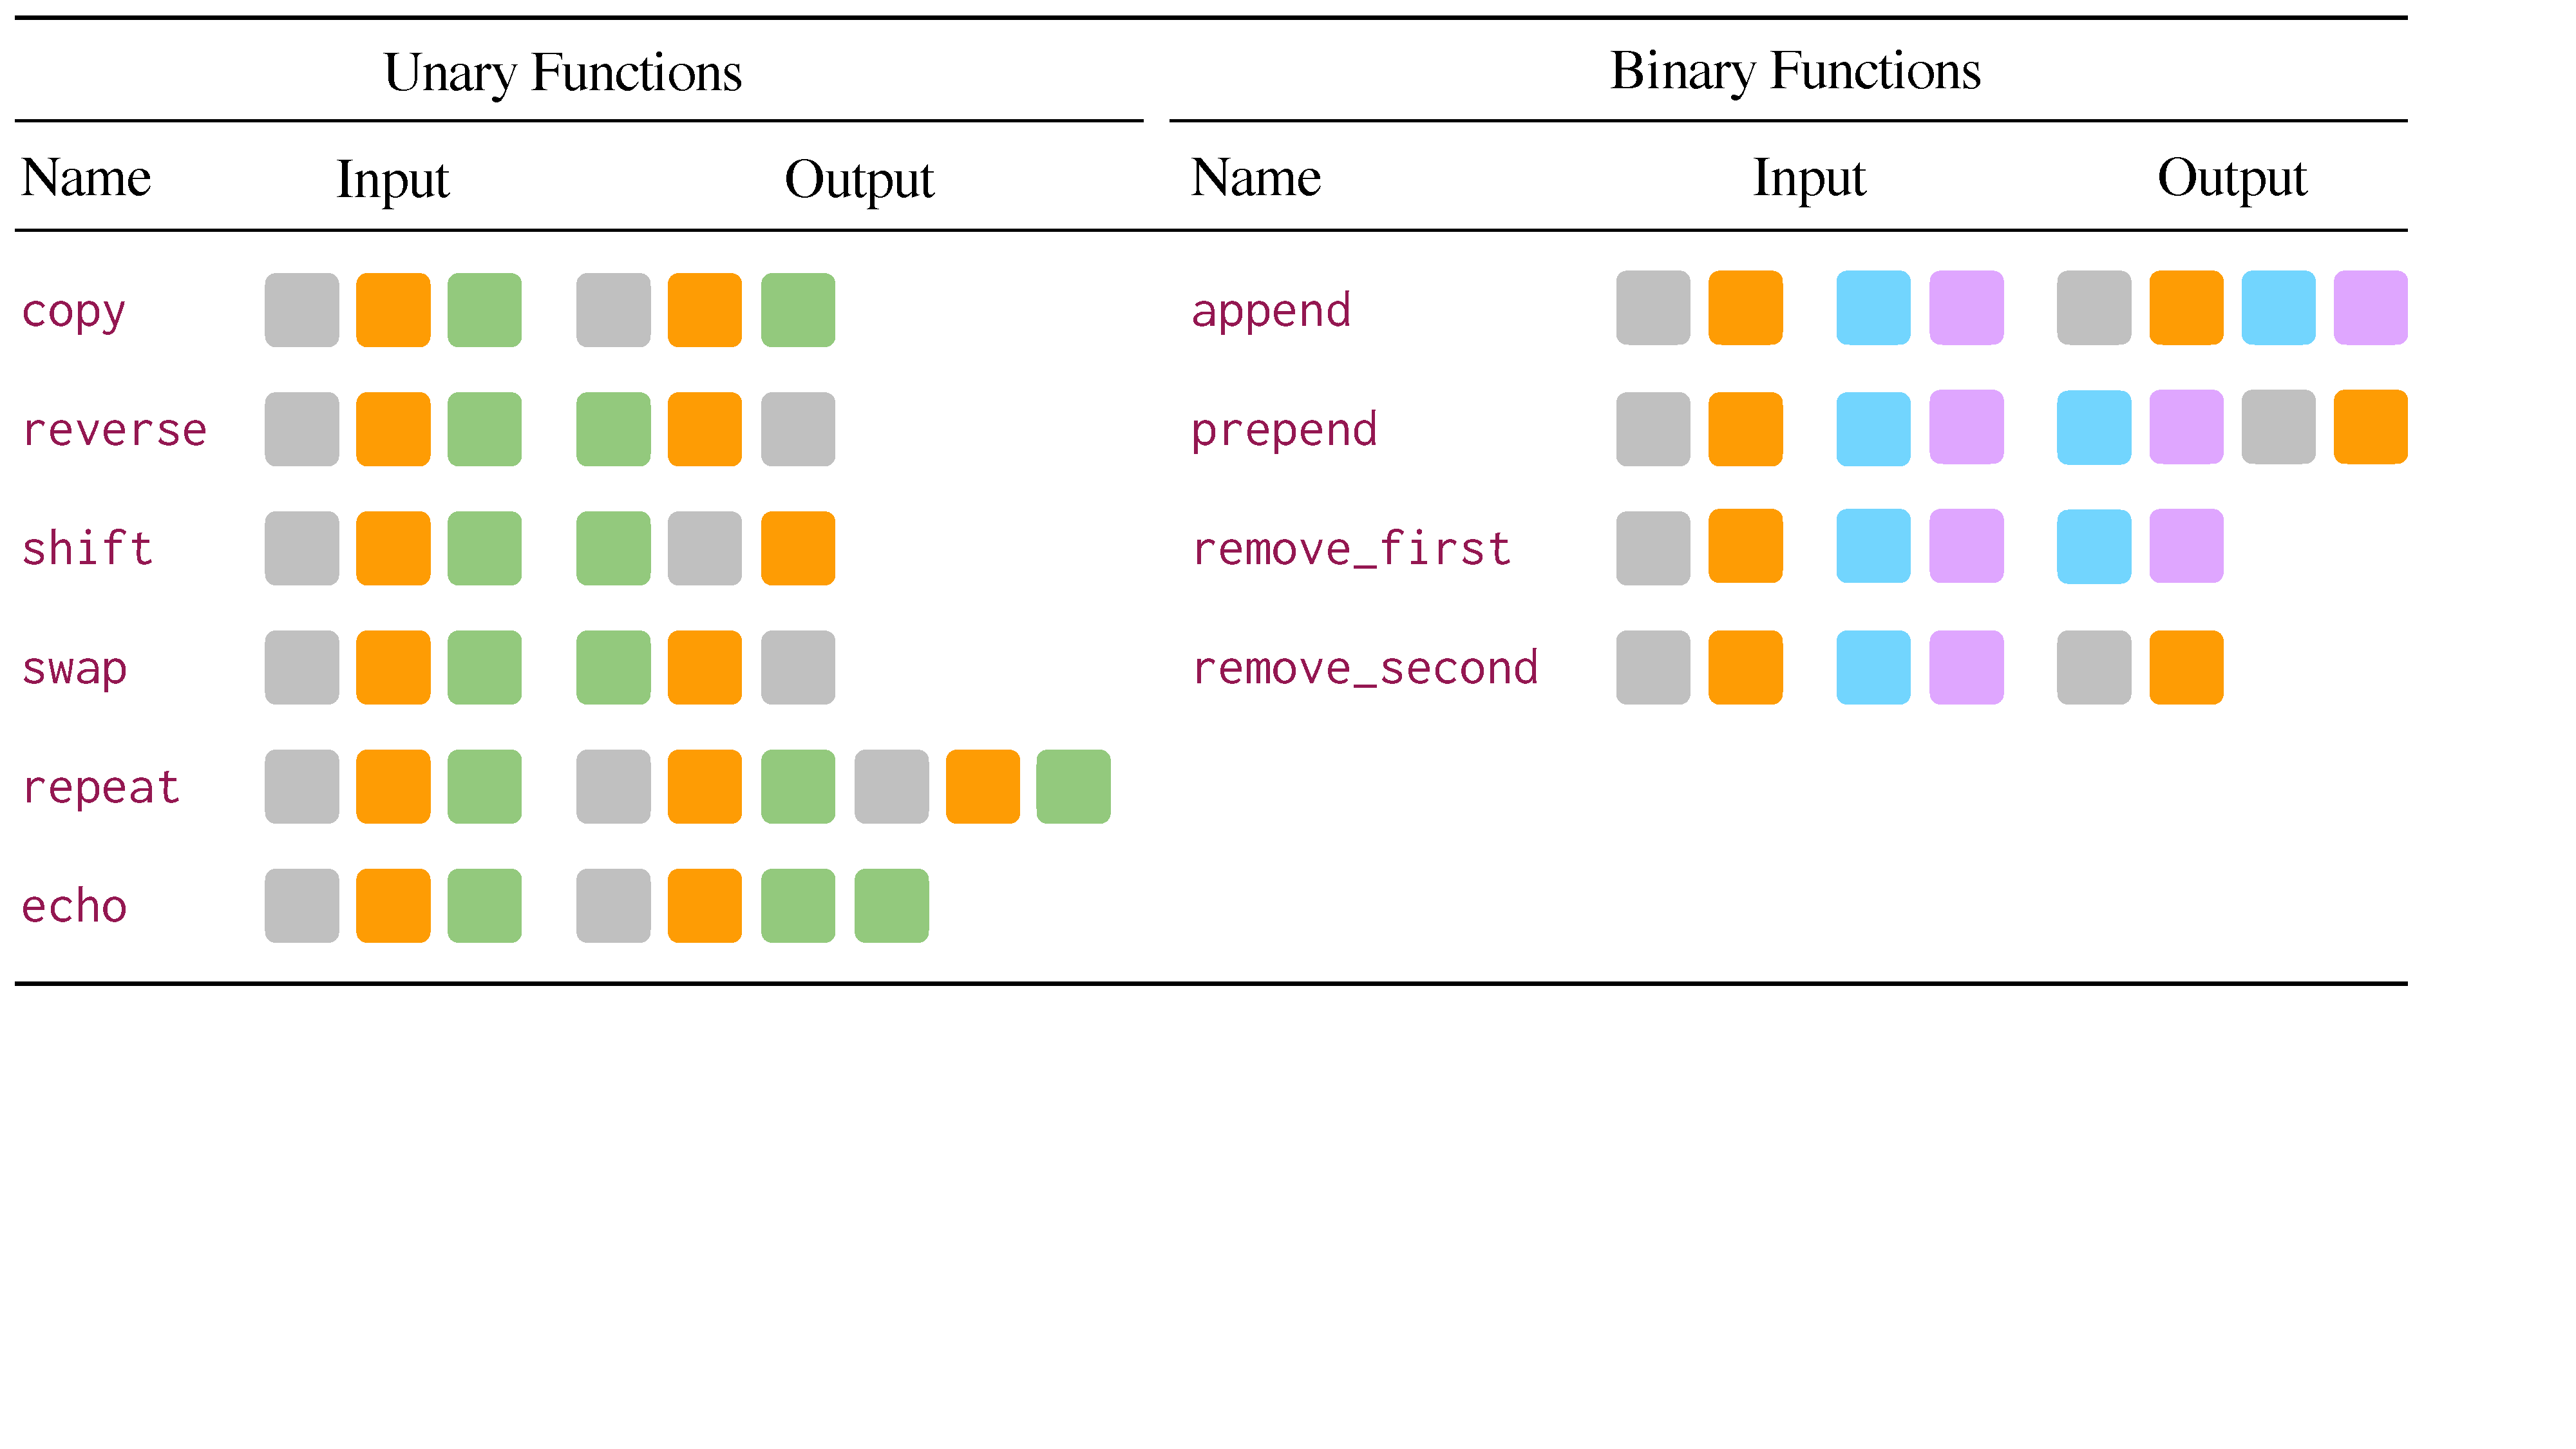
\includegraphics[width=\textwidth]{figures/pcfg-operators.pdf}
    \captionof{table}{\small{Illustrations depicting the unary and binary operators from Hupkes et al. 2020, which we use for our PCFG benchmark.}}
    \label{tab:pcfg-operators}
\end{figure}

\begin{figure}[h]
    \centering
    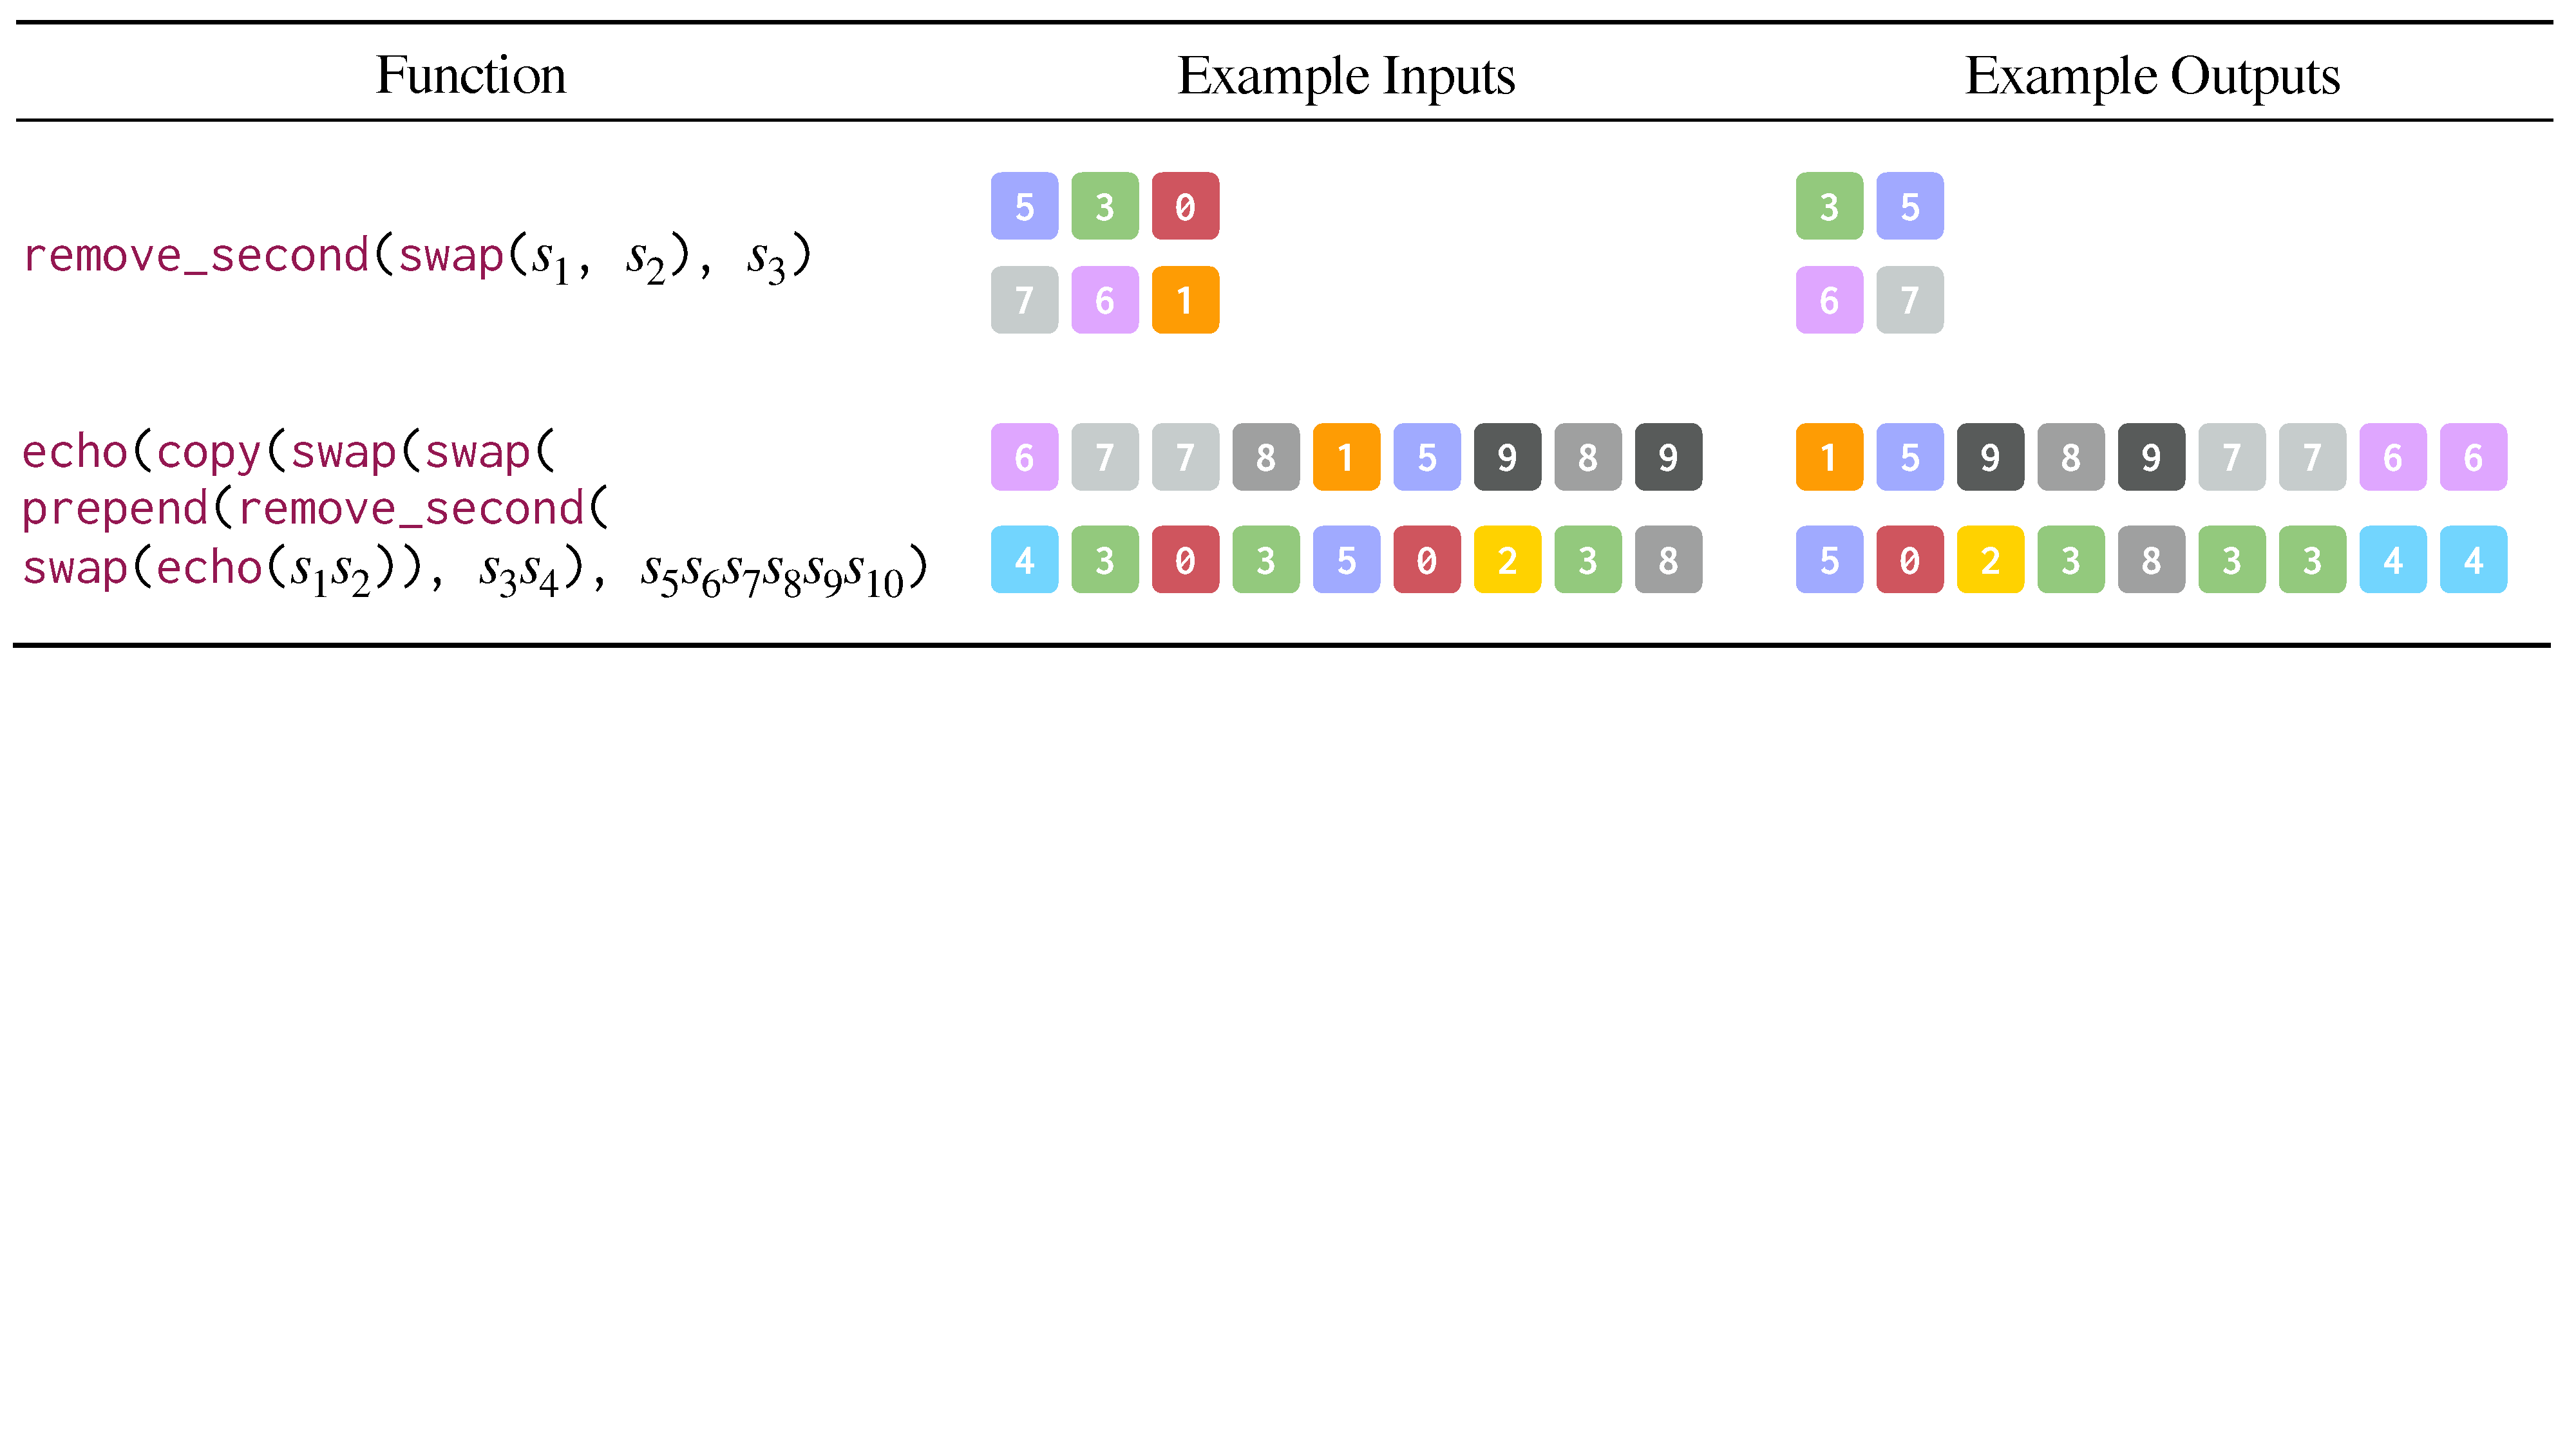
\includegraphics[width=\textwidth]{figures/pcfg-examples.pdf}
    \captionof{table}{\small{Illustrations of transformations in our PCFG benchmark. Row 1 shows a transformation composed of $w=2$ operations over $k=3$ tokens, and row 2 shows a transformation composed of $w=8$ operations over $k=10$ tokens, respectively. For each transformation function, we show two example inputs and the corresponding outputs.}
    }
    \label{tab:pcfg-examples}
\end{figure}

\begin{table}[h]
\parbox{.32\linewidth}{
    \small
    \setlength\tabcolsep{3.5pt}
    \centering
    \begin{tabular}{@{}rcccccc@{}}
    \multicolumn{7}{c}{text-davinci-003} \\
    \toprule
    & \multicolumn{6}{c}{$w$} \\
    \cmidrule(lr){2-7}
    $k$&0&1&3&7&15&31 \\
    \midrule
    1&100&-&-&-&-&- \\
    2&100&100&-&-&-&- \\
    4&100&100&100&-&-&- \\
    8&100&99&95&92&-&- \\
    16&100&86&59&4&47&- \\
    32&100&74&32&14&12&22 \\
    \bottomrule
    \vspace{-0.5em}
    \end{tabular}
    \vspace{-1.0em}
    \label{tab:pcfg-results-kw-davinci}
}
\parbox{.32\linewidth}{
    \small
    \setlength\tabcolsep{3.5pt}
    \centering
    \begin{tabular}{@{}rcccccc@{}}
    \multicolumn{7}{c}{text-davinci-003 w/ random $\mathcal{A}$} \\
    \toprule
    & \multicolumn{6}{c}{$w$} \\
    \cmidrule(lr){2-7}
    $k$&0&1&3&7&15&31 \\
    \midrule
    1&92&-&-&-&-&- \\
    2&91&92&-&-&-&- \\
    4&93&92&93&-&-&- \\
    8&88&82&62&49&-&- \\
    16&84&64&32&17&22&- \\
    32&83&40&13&8&9&12 \\
    \bottomrule
    \vspace{-0.5em}
    \end{tabular}
    \vspace{-1.0em}
    \label{tab:pcfg-results-kw-davinci-rand}
}
\parbox{.32\linewidth}{
    \small
    \setlength\tabcolsep{3.5pt}
    \centering
    \begin{tabular}{@{}rcccccc@{}}
    \multicolumn{7}{c}{PaLM} \\
    \toprule
    & \multicolumn{6}{c}{$w$} \\
    \cmidrule(lr){2-7}
    $k$&0&1&3&7&15&31 \\
    \midrule
    1&100&-&-&-&-&- \\
    2&100&100&-&-&-&- \\
    4&100&100&100&-&-&- \\
    8&100&89&74&82&-&- \\
    16&100&78&57&51&58&- \\
    32&100&68&23&18&22&34 \\
    \bottomrule
    \vspace{-0.5em}
    \end{tabular}
    \vspace{-1.0em}
    \caption{
    \small
    Solve rate (\%) for PCFG across number of tokens $k$ and number of rules $w$ for different models.
    }
    \label{tab:pcfg-results-kw}
}

\end{table}

\begin{lstlisting}[
    basicstyle=\ttfamily\footnotesize,
    backgroundcolor=\color{light},
    breaklines=true,
    caption={\small{Example context format for a PCFG problem (two input-output examples are shown, along with a query input).}},
    captionpos=b,
    label={lst:pcfg-prompt}
    ]
 6 7 7 8 1 5 9 8 9, 1 5 9 8 9 7 7 6 6; 4 3 0 3 5 0 2 3 8; 5 0 2 3 8 3 3 4 4; 1 3 3 3 7 0 1 9 9, 
\end{lstlisting}

\subsection{PCFG Benchmark: Program Synthesis}
\label{app:pcfg-dreamcoder}


We have run DreamCoder \cite{ellis2021dreamcoder} on our PCFG benchmark to contextualize the hardness of the task, and present the results in \cref{tab:pcfg-results-kw-rebuttal}.
We ran DreamCoder with two different sets of initial primitives:
\begin{itemize}[leftmargin=*]
    \item
        \textit{PCFG Ops.}
        In this version, we provide DreamCoder with an initial set of primitives that corresponds to the exact set of unary and binary functions (from \cite{hupkes2020compositionality}) that the PCFG benchmark is based on:
        $\tt{copy}$,
        $\tt{reverse}$,
        $\tt{shift}$,
        $\tt{swap}$,
        $\tt{repeat}$,
        $\tt{echo}$,
        $\tt{append}$,
        $\tt{prepend}$,
        $\tt{remove\_first}$,
        $\tt{remove\_second}$.
        We also include a slicing operator $\texttt{slice}$, $\texttt{length}$, and integers $\tt{1}$--$\tt{10}$.
    \item
        \textit{List Ops.}
        In this version, we provide DreamCoder with a set of list primitives:
        $\tt{length}$,
        $\tt{empty}$,
        $\tt{singleton}$,
        $\tt{range}$,
        $\tt{append}$,
        $\tt{map}$,
        $\tt{reduce}$,
        $\tt{true}$,
        $\tt{not}$,
        $\tt{and}$,
        $\tt{or}$,
        $\tt{sort}$,
        $\tt{add}$,
        $\tt{negate}$,
        $\tt{equal}$,
        $\tt{reverse}$,
        $\tt{index}$,
        $\tt{filter}$,
        $\tt{slice}$. These primitives are not specially designed for PCFG and are based on those used in \cite{ellis2021dreamcoder,ellis2018learning}. 
\end{itemize}

In both cases, the provided primitives are sufficient to define the transformations in the PCFG benchmark.
For each $(k, w)$ pair in \cref{tab:pcfg-results-kw-rebuttal}, we train on 100 task instances and report the number of tasks which get solved (i.e. a correct program that satisfies the training examples is discovered). %
We ran DreamCoder for 4 iterations and use the default hyperparameters and timeout. As we would expect, the version of DreamCoder with ``oracle'' access to the PCFG operations performs well, in several cases matching or exceeding the performance of LLMs. This is especially true when the search problem is easier (i.e. when number of functions $w$ is smaller). The version of DreamCoder with access to list primitives is also able to solve many of the tasks with small values of $w$, but there is a sizeable dropoff as the complexity of the tasks increases. These results help to contextualize the difficulty of the PCFG benchmark when given access to different amounts of domain-specific information. We also note that we would expect brute-force search over the PCFG operators to eventually solve these tasks. Doubling the computation time budget for the version with oracle access to the PCFG operators leads to increased success rates ($k=8$, $w=3$) increases from 80$\rightarrow$84; ($k=16$, $w=7$) increases from 33$\rightarrow$41.

\begin{table}

\parbox{.32\linewidth}{
    \small
    \setlength\tabcolsep{3.5pt}
    \centering
    \begin{tabular}{@{}rcccccc@{}}
    \multicolumn{7}{c}{DreamCoder w/ PCFG Ops.} \\
    \toprule
    & \multicolumn{6}{c}{$w$} \\
    \cmidrule(lr){2-7}
    $k$&0&1&3&7&15&31 \\
    \midrule
     1& 100 & - & - & - & - & -       \\
     2& 100 & 100 & - & - & - & -     \\
     4& 100 & 100 & 98 & - & - & -    \\
     8& 100 & 100 & 80 & 58 & - & -   \\
    16& 100 & 98 & 64 & 38 & 38 & -   \\
    32& 100 & 96 & 41 & 24 & 26 & 37  \\
    \bottomrule
    \vspace{-0.5em}
    \end{tabular}
    \vspace{-1.0em}
}
\parbox{.32\linewidth}{
    \small
    \setlength\tabcolsep{3.5pt}
    \centering
    \begin{tabular}{@{}rcccccc@{}}
    \multicolumn{7}{c}{DreamCoder w/ List Ops.} \\
    \toprule
    & \multicolumn{6}{c}{$w$} \\
    \cmidrule(lr){2-7}
    $k$&0&1&3&7&15&31 \\
    \midrule
     1& 100 & - & - & - & - &    -  \\
     2& 100 & 100 & - & - & - &  -  \\
     4& 100 & 85 & 51 & - & - &  -  \\
     8& 100 & 81 & 23 & 25 & - & -  \\
    16& 100 & 63 & 26 & 4 & 17 & -  \\
    32& 100 & 66 & 6 & 3 & 5 & 11  \\
    \bottomrule
    \vspace{-0.5em}
    \end{tabular}
    \vspace{-1.0em}
    \caption{
    \small
    Solve rate (\%) for PCFG across number of tokens $k$ and number of rules $w$ for DreamCoder initialized with two different sets of primitives.}
    \label{tab:pcfg-results-kw-rebuttal}
}

\end{table}



\section{Sequence Completion}

\subsection{Sinusoids: Structure Learning Comparison}
\label{app:sinusoid-gen}
While the sinusoid extrapolation could be easily performed with standard regression techniques, we contextualize the task with another method that has no specific prior knowledge of the function being extrapolated. We include the structure learning baseline from \cite{cusumano2019gen}, implemented with Gen \cite{cusumano2019gen}. This method uses a Gaussian Process with an inferred covariance kernel to model time series data. The covariance kernel is inferred using MCMC sampling over a PCFG of covariance functions (e.g. squared exponential, periodic). We run the algorithm for 100 iterations and sample from the resulting GP, as shown below in \cref{fig:sinusoids-rebuttal}. The training data is generally fit with low error. However, the quality of the completion differs for the various functions; the sine wave is generally extrapolated well whereas the sinusoids yield high variance samples. Similar to the LLMs, greater context generally yields lower error completions. Note however that the outputs of the structure learning algorithm are high-variance by design, and there are multiple ways to utilize the outputs of the algorithm. We also note that \cite{cusumano2019gen} was tested on a larger set of functions than those we look at here. Though not the goal of our work, it would be interesting future work to evaluate how LLMs extrapolate patterns generated by a wider array of function classes. We also refer to \cite{dinh2022lift} for an extensive comparison of language models to baselines on regression tasks when formulated with a natural language interface as well as a study on the effects of fine-tuning.

\begin{figure}[h]
    \centering
    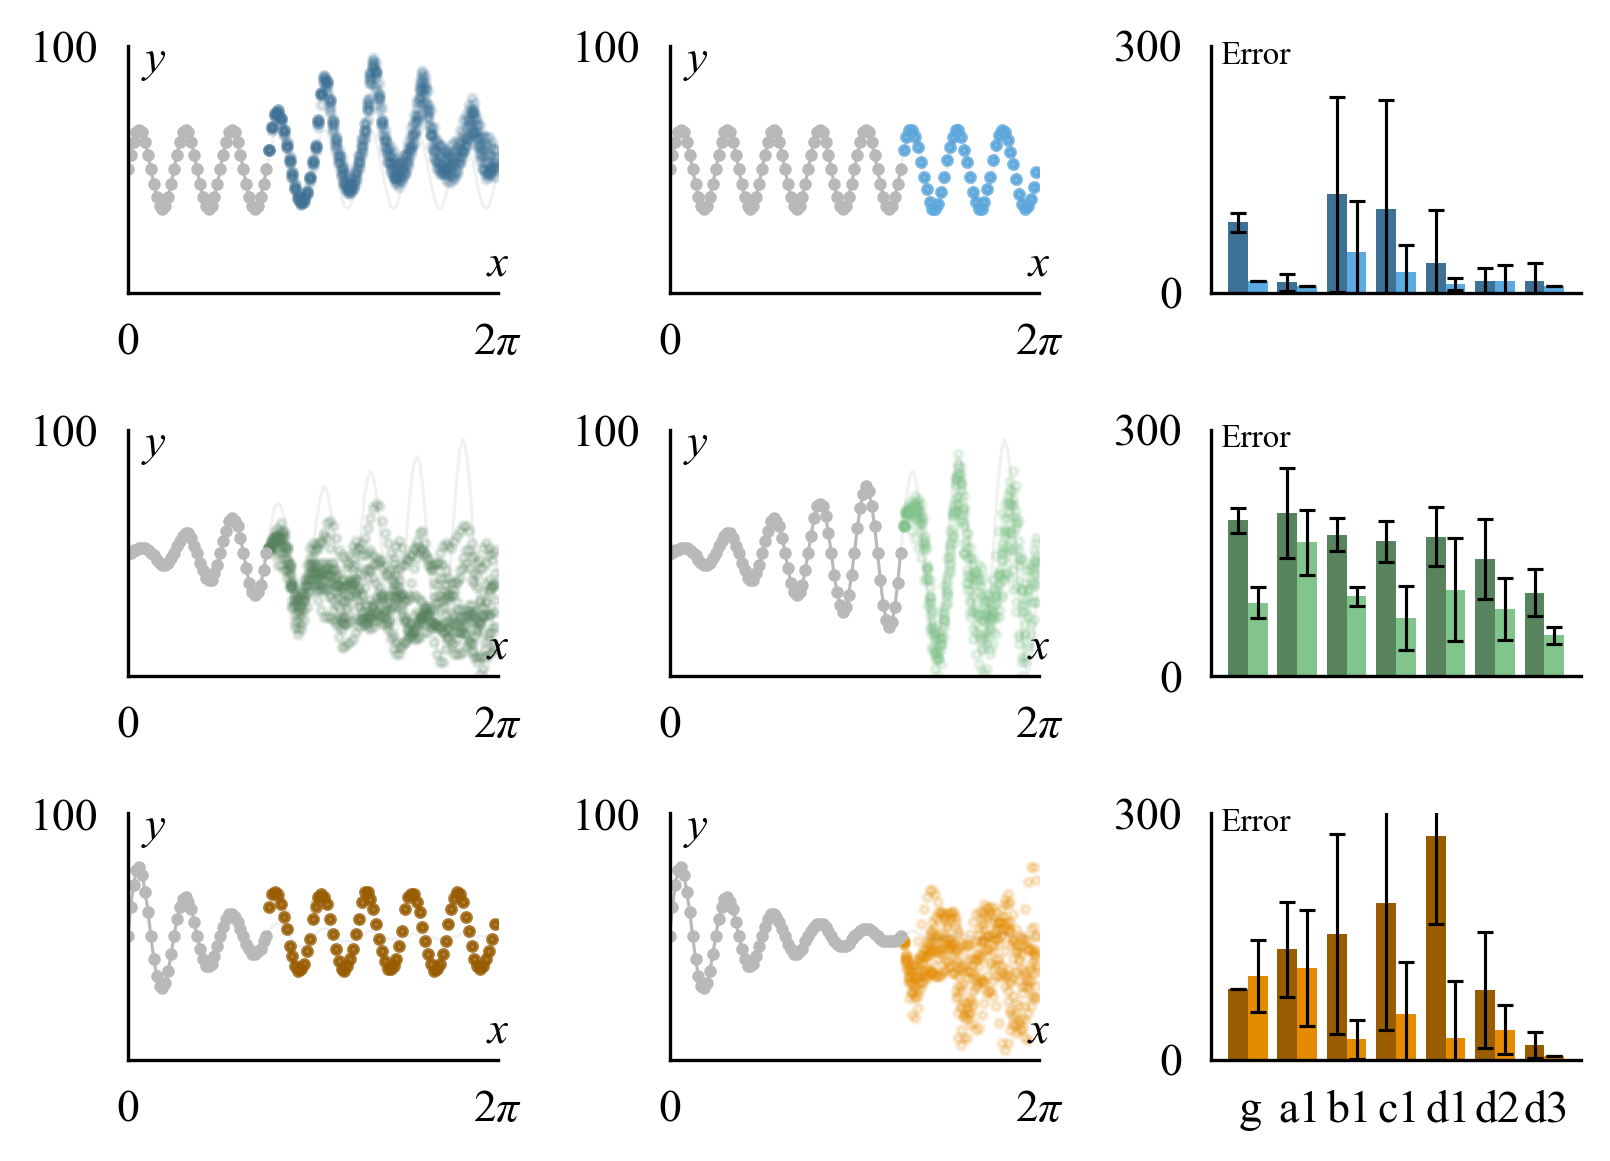
\includegraphics[width=0.5\textwidth]{figures/rebuttal_sinusoids-v1.png}
    \caption{The structure learning approach (g) extrapolates various functions  $y=a\cdot\sin{(bx)}$ (top row), $y=ax\cdot\sin{(bx)}$ (middle row), and $y=\frac{a}{2^x}\sin{(bx)}$ (bottom row) with different degrees of error. More context also generally helps prediction accuracy (light vs. dark).
    }
    \label{fig:sinusoids-rebuttal}
\end{figure}

\subsection{Table Sweeping: Additional Details}

\begin{figure}
    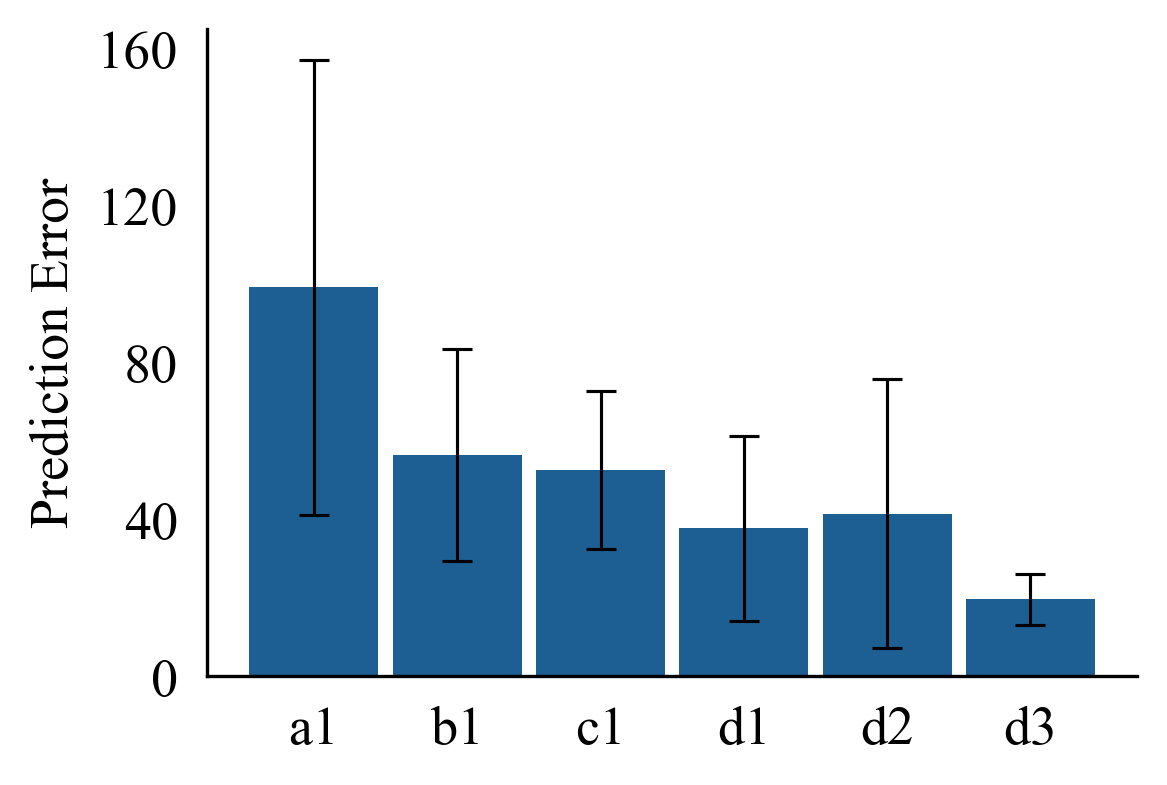
\includegraphics[width=0.4\textwidth]{figures/sweeping-v2.png}
    \caption{
    \small
    LLM trajectory predictions \textit{Table Sweeping} improve with larger models.
    }
    \label{fig:sweeping_extrapolation_dtw}
\end{figure}

In Section 5 of the main paper, we demonstrate how sequence completion capabilities can be applied to continuation of partial motions, such as sweeping a table. In \cref{fig:sweeping_extrapolation_dtw}, we show the average DTW distance between predicted and ground truth trajectory completions in the Table Sweeping task, given 66\% of the trajectory as context, over 30 trials. Each full trajectory consists of 9 sweeping motions across a table. We compare completions made by various language models. We find that larger models generally perform better; text-davinci-003 performs the best, and also has the lowest variance. On our website, we show qualitative examples of text-davinci-003 completing a table sweeping motion given by a human demonstration.

\subsection{Whiteboard Drawing: Qualitative Results}

In \cref{fig:drawing}, we show example completions for three different loop styles by text-davinci-003 over three trials. The completions generally match the overall shape shown in the two loops given as context. However, the results also qualitatively illustrate that fine motion patterns can be challenging to predict precisely.

\begin{figure}[h]
    \centering
    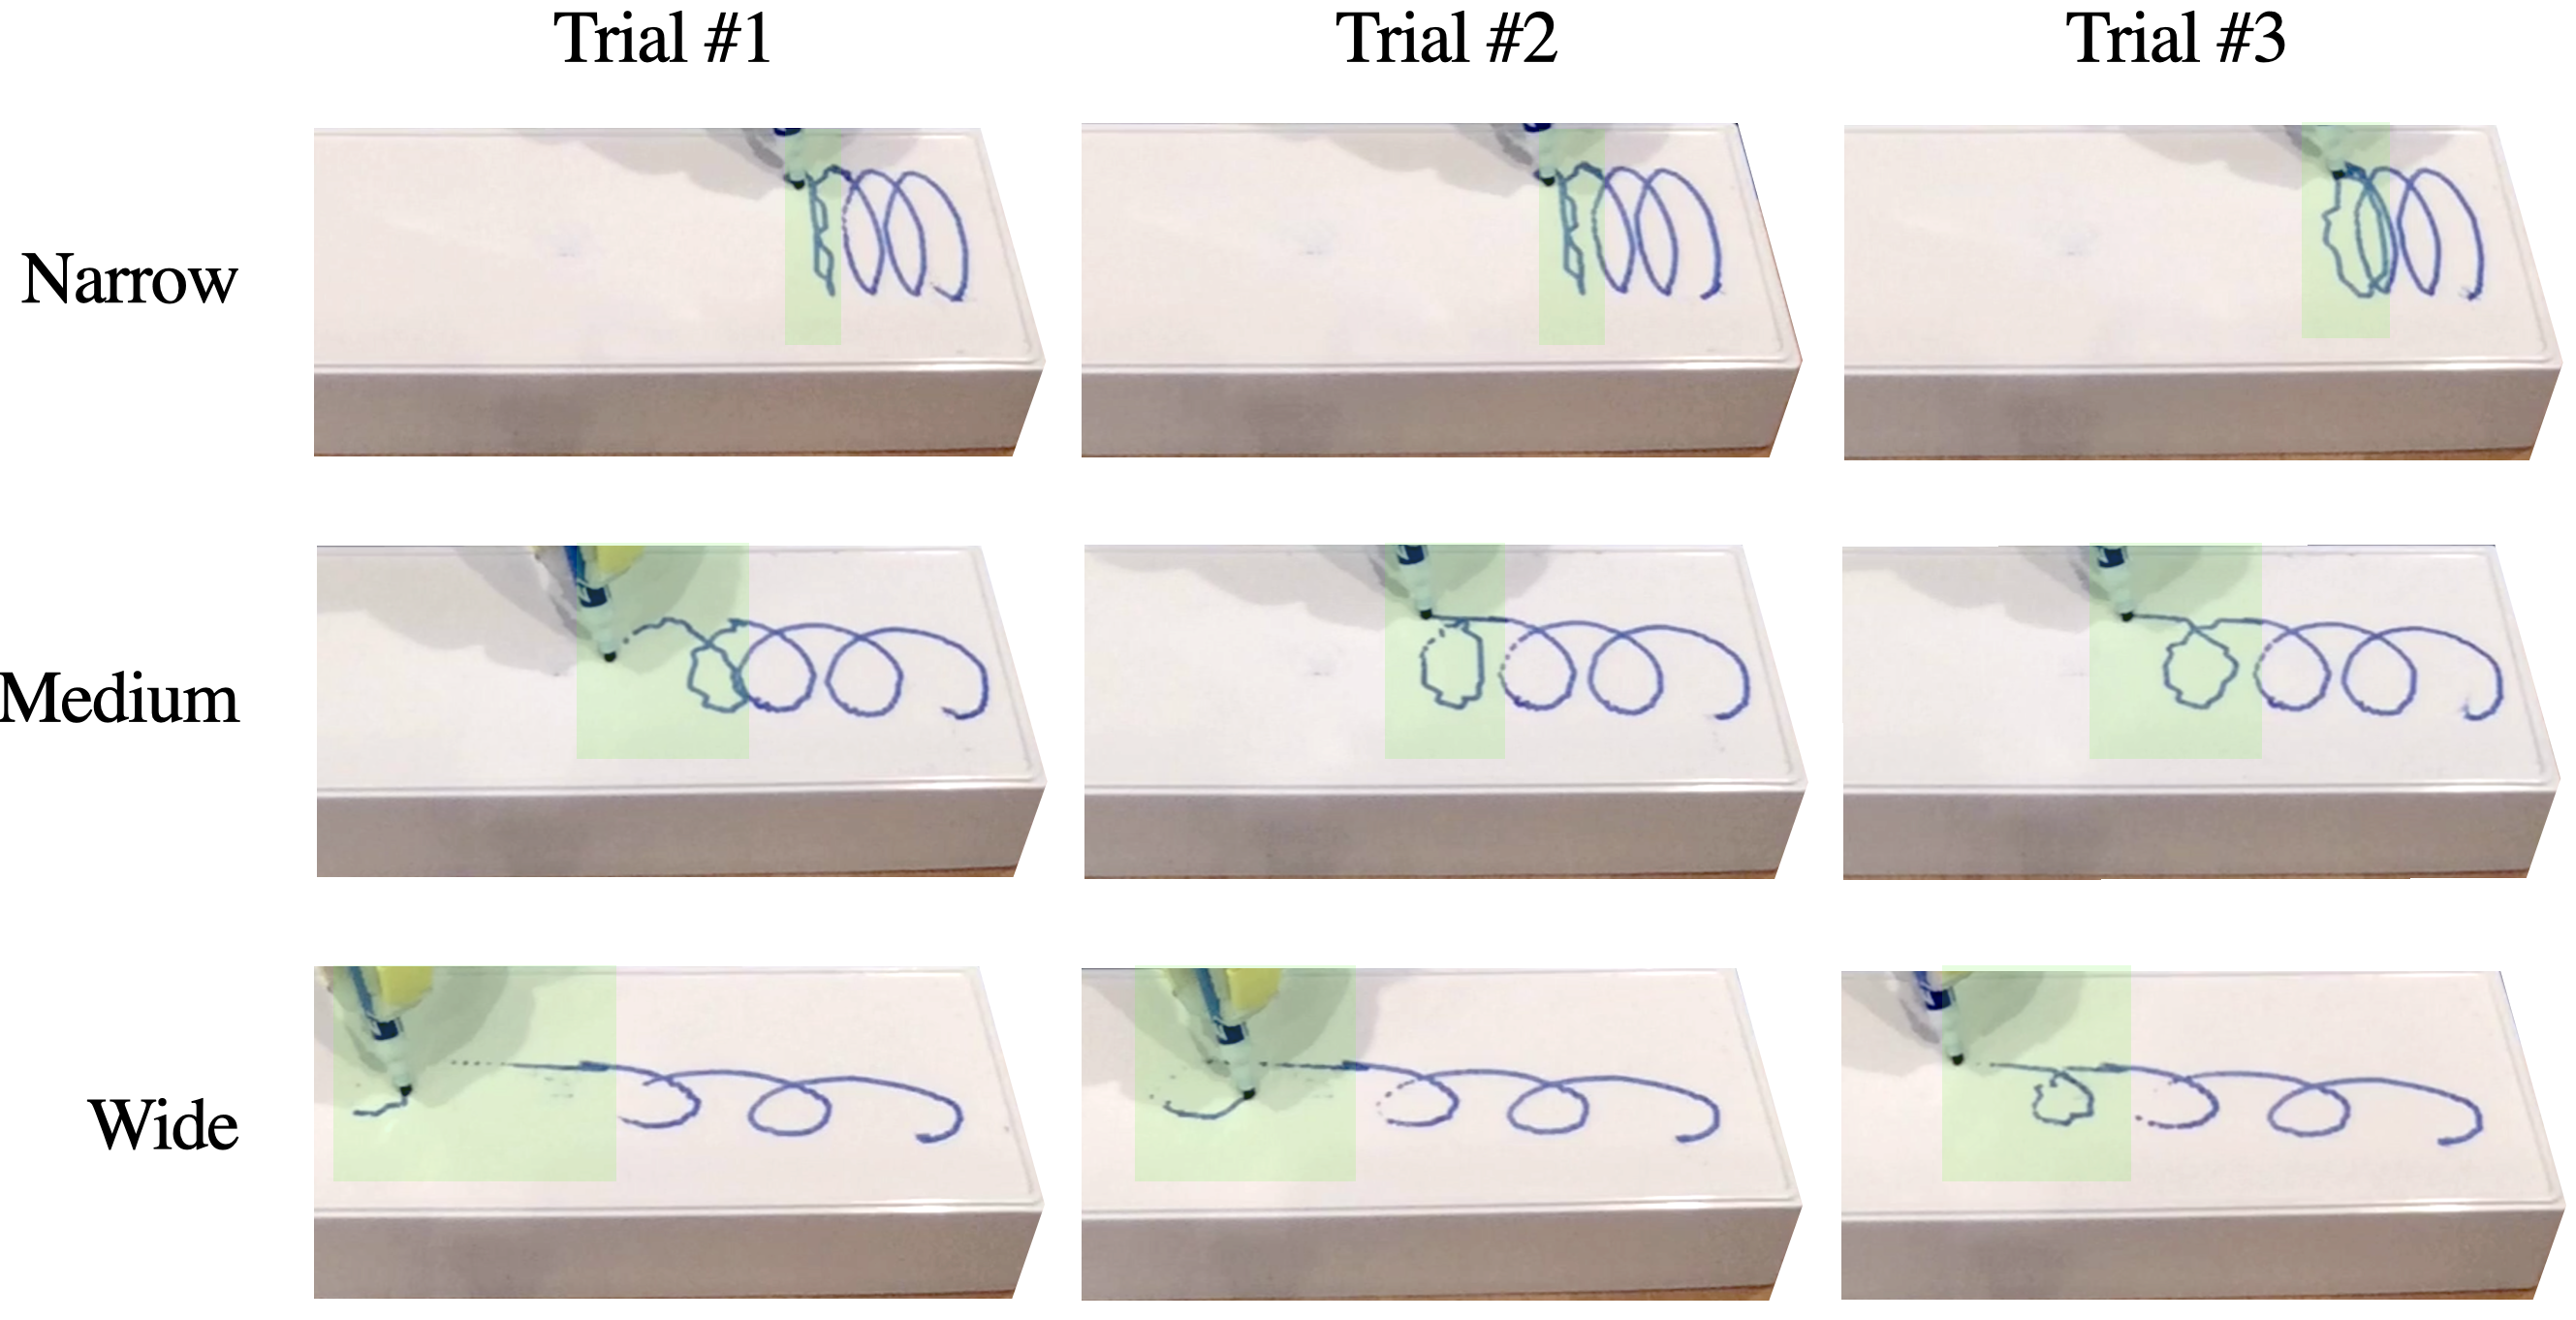
\includegraphics[width=0.7\textwidth]{figures/drawing-v2.png}
    \captionof{figure}{\small{Sampled drawings produced by performing an in-context completion (of one loop, highlighted in green) given a scripted demonstration of two loops. Each row is a different loop style (narrow, medium, wide), and each column is a different trial. Results are shown for text-davinci-003.}}
    \label{fig:drawing}
\end{figure}

\section{Sequence Improvement}

\subsection{Marker in Cup: Additional Details}

In this task, we use LLMs to generate improved trajectories (according to a reward metric) given a context of trajectories that have increasing returns. For this task, states are Cartesian ($x$, $y$, $z$) positions, with each dimension normalized between 0 and 200, trajectories are series of states that can be executed via position control, and the return of a trajectory is proportional to the negative distance to the goal (cup) plus an offset. We form the trajectories in the context as follows: we take a full trajectory which attains a reward of 100 and construct trajectories that stop moving 20\%, 40\%, 60\%, and 80\% of the way to the goal (such that all trajectories are 50 timesteps). We condition the LLM to generate a 100-reward trajectory by prompting it with ``100: \textit{start state}".  An excerpt of an example context is shown in \cref{lst:marker-prompt}. The results in Figure 5 from the main paper are over 11 trials, each with a different goal position.

\begin{lstlisting}[
    basicstyle=\ttfamily\footnotesize,
    backgroundcolor=\color{light},
    breaklines=true,
    caption={\small{Example context (excerpt) for a Marker in Cup, illustrating the (\textit{reward}: \textit{state}, \textit{state}, \textit{state}...) format..}},
    captionpos=b,
    label={lst:marker-prompt}
    ]
71: 104 83 123, 104 83 123, ...
72: 104 83 123, 104 83 123, ...
80: 104 83 123, 104 83 123, ...
90: 104 83 123, 104 83 123, 104 83 123, 104 83 123, 104 83 123, 104 83 123, 104 83 123, 104 83 123, 104 83 123, 104 83 123, 104 83 123, 104 83 123, 104 83 123, 104 83 123, 104 83 123, 105 83 123, 105 83 123, 106 83 123, 106 83 123, 107 83 123, 108 83 122, 109 83 122, 110 83 122, 111 83 121, 112 82 120, 113 82 119, 113 82 118, 114 81 118, 115 81 117, 115 81 116, 115 80 115, 116 80 114, 116 80 113, 117 79 112, 117 79 111, 118 79 110, 118 78 109, 118 78 109, 118 78 109, 118 78 109, 118 78 109, 118 78 109, 118 78 109, 118 78 109, 118 78 109, 118 78 109, 118 78 109, 118 78 109, 118 78 109, 118 78 109
100: 104 83 123
\end{lstlisting}

\subsection{Grid: Additional Details}

In the \textit{Grid} environment, observations are $x, y$ positions represented by integers 0--8 for each coordinate. There are five possible actions (1, 2, 3, 4, 5) corresponding to (right, up, left, down) movement by one space and no-op. A goal is randomly placed in the grid. The agent (which is initialized at the center position) receives a reward of 100 - 10 * distance from the goal to the agent's final position. Episodes terminate after 20 time steps. For our experiments, we limit the context length to 1024 tokens. At each iteration, the LLMs is prompted to generate a trajectory with the maximum seen return from the buffer plus a randomly selected offset of up to 20.



\subsection{CartPole: Additional Details}

We use a simplified version of the CartPole enviornment in OpenAI Gym. Observations are two-dimensional (corresponding to pole angle and velocity, normalized to 0-100) and the maximum time horizon is 200. There are two possible actions (1, 2) corresponding to (left, right), and the agent gets +1 reward for every time step that the CartPole is kept upright. In \cref{lst:cartpole-prompt}, we show an example context excerpt for CartPole, where a trajectory history is appended with an encoding of the current trajectory.

\begin{lstlisting}[
    basicstyle=\ttfamily\footnotesize,
    backgroundcolor=\color{light},
    breaklines=true,
    caption={\small{ Example context format for a CartPole run. A trajectory history (with each trajectory in the format \textit{reward}: \textit{observation}, \textit{action}, \textit{observation}, \textit{action} ...) is followed by an encoding of the current trajectory, up to the current observation.}},
    captionpos=b,
    label={lst:cartpole-prompt}
    ]
52: 40 50, 1, 40 54, 2, 41 49, 1, 41 54, 1, ...
60: 45 50, 2, 45 45, 1, 44 50, 2, 44 45, 1, ...
75: 52 50, 1, 52 55, 2, 53 50, 2, 53 46, 2, ...
98: 44 50, 1, 44 55, 2, 45 50, 
\end{lstlisting}

Below, we discuss some additional considerations for forming the context from the trajectory history.

\textit{Context Length}. When context length is longer, more trajectories can fit in the context (which yields more in-context ``training data" that could potentially be used to generalize to higher rewards, but also requires the LLM to attend over more tokens). Context length is a limiting factor of using current LLMs in our trajectory improvement setting: the number of tokens required to represent a trajectory history scales with the observation dimensionality, action dimensionality, time horizon, and number of trajectories. For our CartPole experiments, we limit the context to 1024 tokens (which is the maximum context length for text-ada-001, text-babbage-001, and text-curie-001 models). 

\textit{Action Representation}. In initial experiments, we found that the tokens used to represent the action space (e.g. ``0" for left, ``1" for right) can seemingly affect the ability of an LLM to improve trajectories in the online setting. For example, we observed that if ``0" is included in the action space, LLMs may ``default" to sampling ``0" (likely due to token-specific priors). Therefore, for our experiments, we use 1-indexed integer action representations, which appears to alleviate the bias towards choosing a particular action. The fact that action representation can sometimes affect performance complements our observations in the Sequence Transformation section, in which we find that token mapping invariance holds to some extent, but not entirely.

\subsection{Clicker Training: Additional Details}

In our clicker training example, the observation consists of the end-effector position and the approximate object position as determined by visual input, with the $(x,y,z)$ values normalized between 0 and 300. Actions correspond to movements of the end-effector (normalized between 0 and 100, such that \tt{50,50,50} represents no movement). A sample context is given in \cref{lst:clicker-prompt}.

\begin{lstlisting}[
    basicstyle=\ttfamily\footnotesize,
    backgroundcolor=\color{light},
    breaklines=true,
    caption={\small{ Example context format for clicker training. (\textit{Reward}, \textit{observation}, \textit{action}) tuples are ordered by reward (with a click corresponding to a reward of 1) with an equal number of reward 0 and reward 1 transitions represented in the context.}}, 
    captionpos=b,
    label={lst:clicker-prompt}
    ]
0: 80,49,138,109,54,133; 45,44,55
0: 82,32,155,109,54,133; 48,59,48
0: 82,32,155,109,54,133; 48,59,48
1: 88,31,154,109,54,133; 45,54,43
1: 85,36,146,109,54,133; 57,54,46
1: 93,40,142,109,54,133; 44,52,43
1: ...
\end{lstlisting}
